
\let\negmedspace\undefined
\let\negthickspace\undefined
\documentclass[journal]{IEEEtran}
\usepackage[a5paper, margin=10mm, onecolumn]{geometry}
%\usepackage{lmodern} % Ensure lmodern is loaded for pdflatex
\usepackage{tfrupee} % Include tfrupee package

\setlength{\headheight}{1cm} % Set the height of the header box
\setlength{\headsep}{0mm}     % Set the distance between the header box and the top of the text

\usepackage{gvv-book}
\usepackage{gvv}
\usepackage{cite}
\usepackage{amsmath,amssymb,amsfonts,amsthm}
\usepackage{algorithmic}
\usepackage{graphicx}
\usepackage{textcomp}
\usepackage{xcolor}
\usepackage{txfonts}
\usepackage{listings}
\usepackage{enumitem}
\usepackage{mathtools}
\usepackage{gensymb}
\usepackage{comment}
\usepackage[breaklinks=true]{hyperref}
\usepackage{tkz-euclide} 
\usepackage{listings}
% \usepackage{gvv}                                        
\def\inputGnumericTable{}                                 
\usepackage[latin1]{inputenc}                                
\usepackage{color}                                            
\usepackage{array}                                            
\usepackage{longtable}                                       
\usepackage{calc}                                             
\usepackage{multirow}                                         
\usepackage{hhline}                                           
\usepackage{ifthen}                                           
\usepackage{lscape}
\begin{document}

\bibliographystyle{IEEEtran}
\vspace{3cm}
\title{1.4.9.d}
\author{EE24BTECH11025 - GEEDI HARSHA}
% \maketitle
% \newpage
{\let\newpage\relax\maketitle}

\renewcommand{\thefigure}{\theenumi}
\renewcommand{\thetable}{\theenumi}
\setlength{\intextsep}{10pt} % Space between text and floats


\numberwithin{equation}{enumi}
\numberwithin{figure}{enumi}
\renewcommand{\thetable}{\theenumi}

\textbf{Question:}Which of the following differential equations has $y = C_1 e^x + C_2 e^{-x}$ as the general solution?\\

\begin{align}
\text{(D) } \frac{d^2y}{dx^2} - 1 = 0
\end{align}



\solution

First, Plot the graph of $y = C_1 e^x + C_2 e^{-x}$

Consider,
\begin{align}
\frac{d^2y}{dx^2} = 1 \label{2}
\end{align}
On integrating both sides w.r.to x
\begin{align}
\int \frac{d^2y}{dx^2} dx = \int 1 dx \\
\frac{dy}{dx} = x + C_1
\end{align}
Again integrating on both sides w.r.to x
\begin{align}
\int \frac{dy}{dx} dx = \int \brak{x + C_1} dx \\
y = \frac{x^2}{2}+C_1x+C_2
\end{align}
Where,$C_1,C_2$ are integration constants.
Now lets plot $y = \frac{x^2}{2}+C_1x+C_2 $ in the same graph.\\ 

Solution using Laplace Transform:\\

Laplace Transform definition\\
\begin{align}
    \mathcal{L}\brak{f\brak{t}} = F(s) = \int_{0}^{\infty}e^{-st}f\brak{t}dt
\end{align}
Properties of Laplace transform
\begin{align}
    \mathcal{L}\brak{y^{\prime\prime}} &= s^2F(s) - sy\brak{0} - y^\prime\brak{0}\\
    \mathcal{L}\brak{1} &= \frac{1}{s}\\
    \mathcal{L}^{-1}\brak{\frac{2}{s^3}} &= x^2u\brak{x}\\
    \mathcal{L}\brak{cf\brak{t}} &= cF(s)
\end{align}
Applying the properties to the given equation
\begin{align}
    y^{\prime\prime} &= 1\\
    \mathcal{L}\brak{y^{\prime\prime}} &= \mathcal{L}\brak{1}\\
    s^2F(s) - sy\brak{0} - y^\prime\brak{0} &= \frac{1}{s}
\end{align}
Substituting the initial conditions \(y(0) = 0\) and \(y^\prime(0) = 0\), we get
\begin{align}
    s^2F(s) &= \frac{1}{s}\\
    F(s) &= \frac{1}{s^3}
\end{align}
\textbf{Region of Convergence (ROC):} The ROC for \(F(s) = \frac{1}{s^3}\) is \(s > 0\).\\

Obtaining the inverse Laplace transform:
\begin{align}
    y &= \mathcal{L}^{-1}\brak{F(s)}\\
    y &= \mathcal{L}^{-1}\brak{\frac{1}{s^3}}\\
    y &= \frac{1}{2}\mathcal{L}^{-1}\brak{\frac{2}{s^3}}\\
    y &= \frac{1}{2}x^2u\brak{x}
\end{align}

\textbf{Solving the Difference Equation using Z-Transform:}\\
Let the difference equation be:
\[
y[n+2] = 1
\]
Taking the Z-transform of both sides:
\begin{align}
    Z\brak{y[n+2]} &= Z\brak{1}\\
    z^2Y(z) - z^2y[0] - zy[1] &= \frac{z}{z-1}
\end{align}
Substituting the initial conditions \(y[0] = 0\) and \(y[1] = 0\), we get:
\begin{align}
    z^2Y(z) &= \frac{z}{z-1}\\
    Y(z) &= \frac{z}{z^2(z-1)}
\end{align}
The ROC is \(|z| > 1\).\\

Performing partial fraction decomposition:
\begin{align}
    Y(z) &= \frac{A}{z} + \frac{B}{z^2} + \frac{C}{z-1}\\
    &= \frac{1}{z} + \frac{0}{z^2} + \frac{1}{z-1}
\end{align}
Taking the inverse Z-transform:
\begin{align}
    y[n] &= \mathcal{Z}^{-1}\brak{\frac{1}{z}} + \mathcal{Z}^{-1}\brak{\frac{1}{z-1}}\\
    y[n] &= u[n] + nu[n]
\end{align}
Thus, the solution using Z-transform is:
\begin{align}
    y[n] = (1+n)u[n]
\end{align}




\textbf{Using difference equation to find solution for this differential equation}
This method is used to find the approximate solution for the differential equation by plotting the discret points of the function.\\
From defination of second order differentiation,
\begin{align}
\frac{d^2y}{dx^2} = \lim\limits_{h \to 0} \frac{y\brak{x_i+h}-2y\brak{x_i}+y\brak{x_i-h}}{h^2}
\end{align}
\begin{align}
\frac{d^2y}{dx^2} \approx \frac{y\brak{x_i+h}-2y\brak{x_i}+y\brak{x_i-h}}{h^2}
\end{align}
From \eqref{2} \\
\begin{align}
\frac{d^2y}{dx^2} = 1 
\end{align}
\begin{align}
1 = \frac{y_{n+1}-2y_n+y_{n-1}}{h^2} \\
h^2 = y_{n+1}-2y_n+y_{n-1} \\
y_{n+1} = 2y_n-y_{n-1}+h^2 
\end{align}
Let $(x_0,y_0)$, be points on the function
\begin{align}
x_{n+1}=x_{n}+h \\
y_{n+1} = 2y_n-y_{n-1}+h^2 
\end{align}
By taking initial conditions as $y_0 = 0$ at $x_0 = 0$ , $h=0.1$ and running this algorithm,We can get the approximatet plot of the solution of the given differential equation.\\
This is done by plotting all the (x.y) points at different n,and joining all these points.

\begin{figure}[h]
    \centering
    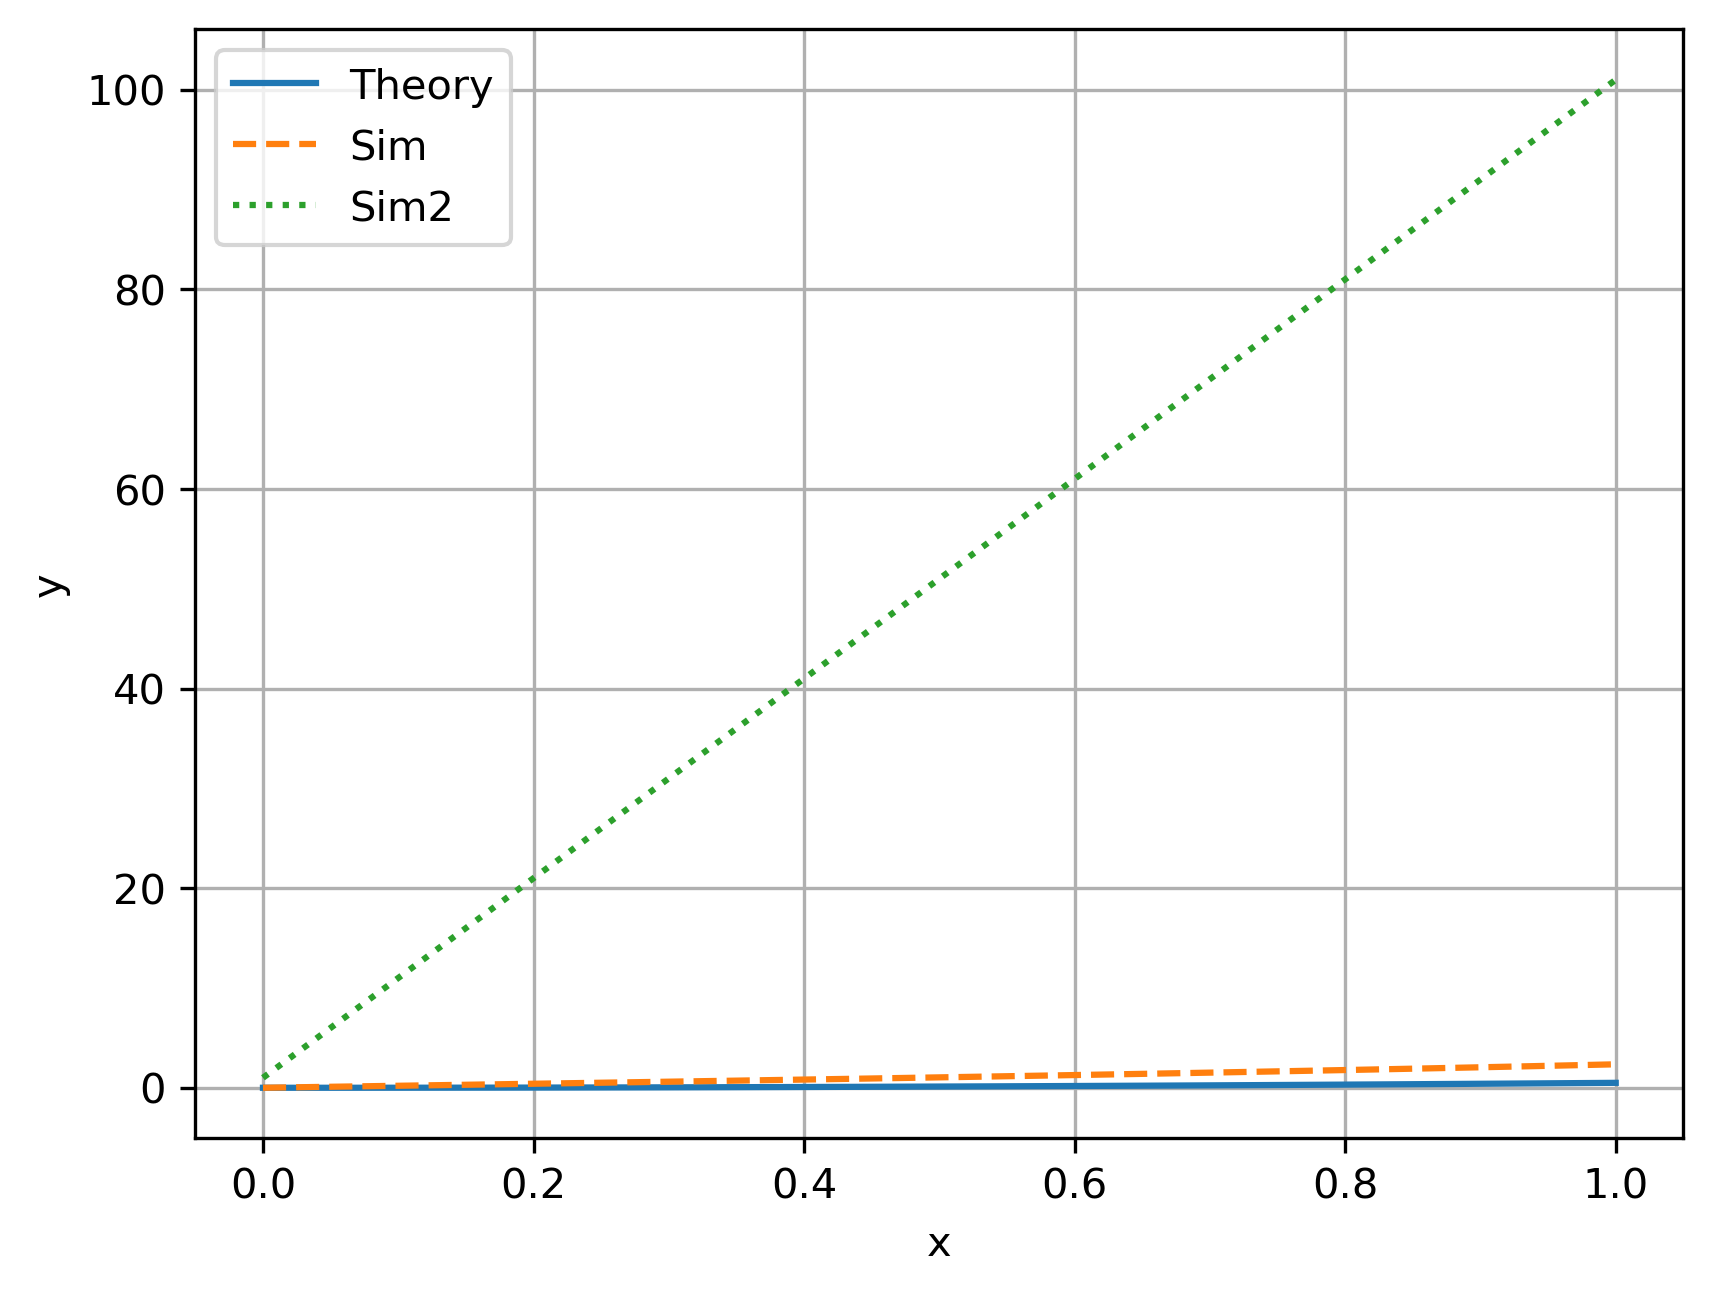
\includegraphics[width=\textwidth]{figs/fig.png}
\end{figure}

As both the plots are not same, Option D is not the solution. \\


\end{document}

